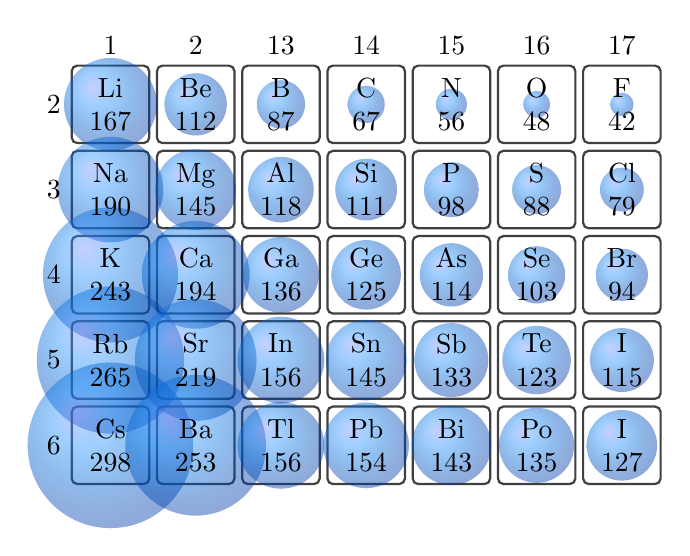
\begin{tikzpicture}
  \def\sep{2pt} % Node distance
  \tikzset
    {
      element/.style = 
        {
          rectangle,
          rounded corners = 2pt,
          thick,
          draw = black!75,
          minimum size = 2.8em,
        },
      atom-radius/.style = 
        {
          nearly transparent, 
          fill = blue,
          ball color = cyan,
        },
    }  

  \begin{scope}[every node/.style = {element}]
    % GRUPO 1
    \node (Li) {};
    \node (Na) [anchor = north, yshift = -\sep] at (Li.south) {};
    \node (K) [anchor = north, yshift = -\sep] at (Na.south) {};
    \node (Rb) [anchor = north, yshift = -\sep] at (K.south) {};
    \node (Cs) [anchor = north, yshift = -\sep] at (Rb.south) {};

    % GRUPO 2
    \node (Be) [anchor = west, xshift = \sep] at (Li.east) {};
    \node (Mg) [anchor = north, yshift = -\sep] at (Be.south) {};
    \node (Ca) [anchor = north, yshift = -\sep] at (Mg.south) {};
    \node (Sr) [anchor = north, yshift = -\sep] at (Ca.south) {};
    \node (Ba) [anchor = north, yshift = -\sep] at (Sr.south) {};

    % GRUPO 13
    \node (B) [anchor = west, xshift = \sep] at (Be.east) {};
    \node (Al) [anchor = north, yshift = -\sep] at (B.south) {};
    \node (Ga) [anchor = north, yshift = -\sep] at (Al.south) {};
    \node (In) [anchor = north, yshift = -\sep] at (Ga.south) {};
    \node (Tl) [anchor = north, yshift = -\sep] at (In.south) {};

    % GRUPO 14
    \node (C) [anchor = west, xshift = \sep] at (B.east) {};
    \node (Si) [anchor = north, yshift = -\sep] at (C.south) {};
    \node (Ge) [anchor = north, yshift = -\sep] at (Si.south) {};
    \node (Sn) [anchor = north, yshift = -\sep] at (Ge.south) {};
    \node (Pb) [anchor = north, yshift = -\sep] at (Sn.south) {};

    % GRUPO 15
    \node (N) [anchor = west, xshift = \sep] at (C.east) {};
    \node (P) [anchor = north, yshift = -\sep] at (N.south) {};
    \node (As) [anchor = north, yshift = -\sep] at (P.south) {};
    \node (Sb) [anchor = north, yshift = -\sep] at (As.south) {};
    \node (Bi) [anchor = north, yshift = -\sep] at (Sb.south) {};

    % GRUPO 16
    \node (O) [anchor = west, xshift = \sep] at (N.east) {};
    \node (S) [anchor = north, yshift = -\sep] at (O.south) {};
    \node (Se) [anchor = north, yshift = -\sep] at (S.south) {};
    \node (Te) [anchor = north, yshift = -\sep] at (Se.south) {};
    \node (Po) [anchor = north, yshift = -\sep] at (Te.south) {};

    % GRUPO 17
    \node (F) [anchor = west, xshift = \sep] at (O.east) {};
    \node (Cl) [anchor = north, yshift = -\sep] at (F.south) {};
    \node (Br) [anchor = north, yshift = -\sep] at (Cl.south) {};
    \node (I) [anchor = north, yshift = -\sep] at (Br.south) {};
    \node (At) [anchor = north, yshift = -\sep] at (I.south) {};
  \end{scope}

  % RAIOS ATÔMICOS
  \fill [atom-radius] (Li) circle (16.7bp);
  \fill [atom-radius] (Na) circle (19.0bp);
  \fill [atom-radius] (K)  circle (24.3bp);
  \fill [atom-radius] (Rb) circle (26.5bp);
  \fill [atom-radius] (Cs) circle (29.8bp);

  \fill [atom-radius] (Be) circle (11.2bp);
  \fill [atom-radius] (Mg) circle (14.5bp);
  \fill [atom-radius] (Ca) circle (19.4bp);
  \fill [atom-radius] (Sr) circle (21.9bp);
  \fill [atom-radius] (Ba) circle (25.3bp);

  \fill [atom-radius] (B)  circle (8.7bp);
  \fill [atom-radius] (Al) circle (11.8bp);
  \fill [atom-radius] (Ga) circle (13.6bp);
  \fill [atom-radius] (In) circle (15.6bp);
  \fill [atom-radius] (Tl) circle (15.6bp);

  \fill [atom-radius] (C)  circle (6.7bp);
  \fill [atom-radius] (Si) circle (11.1bp);
  \fill [atom-radius] (Ge) circle (12.5bp);
  \fill [atom-radius] (Sn) circle (14.5bp);
  \fill [atom-radius] (Pb) circle (15.4bp);

  \fill [atom-radius] (N)  circle (5.6bp);
  \fill [atom-radius] (P)  circle (9.9bp);
  \fill [atom-radius] (As) circle (11.4bp);
  \fill [atom-radius] (Sb) circle (13.3bp);
  \fill [atom-radius] (Bi) circle (14.3bp);

  \fill [atom-radius] (O)  circle (4.8bp);
  \fill [atom-radius] (S)  circle (8.8bp);
  \fill [atom-radius] (Se) circle (10.3bp);
  \fill [atom-radius] (Te) circle (12.3bp);
  \fill [atom-radius] (Po) circle (13.5bp);
  
  \fill [atom-radius] (F)  circle (4.2bp);
  \fill [atom-radius] (Cl) circle (7.9bp);
  \fill [atom-radius] (Br) circle (9.4bp);
  \fill [atom-radius] (I)  circle (11.5bp);
  \fill [atom-radius] (At) circle (12.7bp);

  % LABELS GRUPO
  \begin{scope}[anchor = south]
    \node at (Li.north) {1};
    \node at (Be.north) {2};
    \node at (B.north)  {13};
    \node at (C.north)  {14};
    \node at (N.north)  {15};
    \node at (O.north)  {16};
    \node at (F.north)  {17};
  \end{scope}

  % LABELS PERÍODO
  \begin{scope}[anchor = east]
    \node at (Li.west) {2};
    \node at (Na.west) {3};
    \node at (K.west)  {4};
    \node at (Rb.west) {5};
    \node at (Cs.west) {6};
  \end{scope}

  % LABELS ÁTOMOS
  \begin{scope}[align = center]
    \node at (Li) { \ce{Li} \\ \num{167} };
    \node at (Na) { \ce{Na} \\ \num{190} };
    \node at (K)  { \ce{K}  \\ \num{243} };
    \node at (Rb) { \ce{Rb} \\ \num{265} };
    \node at (Cs) { \ce{Cs} \\ \num{298} };

    \node at (Be) { \ce{Be} \\ \num{112} };
    \node at (Mg) { \ce{Mg} \\ \num{145} };
    \node at (Ca) { \ce{Ca} \\ \num{194} };
    \node at (Sr) { \ce{Sr} \\ \num{219} };
    \node at (Ba) { \ce{Ba} \\ \num{253} };

    \node at (B)  { \ce{B}  \\ \num{87} };
    \node at (Al) { \ce{Al} \\ \num{118} };
    \node at (Ga) { \ce{Ga} \\ \num{136} };
    \node at (In) { \ce{In} \\ \num{156} };
    \node at (Tl) { \ce{Tl} \\ \num{156} };

    \node at (C)  { \ce{C}  \\ \num{67} };
    \node at (Si) { \ce{Si} \\ \num{111} };
    \node at (Ge) { \ce{Ge} \\ \num{125} };
    \node at (Sn) { \ce{Sn} \\ \num{145} };
    \node at (Pb) { \ce{Pb} \\ \num{154} };

    \node at (N)  { \ce{N}  \\ \num{56} };
    \node at (P)  { \ce{P}  \\ \num{98} };
    \node at (As) { \ce{As} \\ \num{114} };
    \node at (Sb) { \ce{Sb} \\ \num{133} };
    \node at (Bi) { \ce{Bi} \\ \num{143} };

    \node at (O)  { \ce{O}  \\ \num{48} };
    \node at (S)  { \ce{S}  \\ \num{88} };
    \node at (Se) { \ce{Se} \\ \num{103} };
    \node at (Te) { \ce{Te} \\ \num{123} };
    \node at (Po) { \ce{Po} \\ \num{135} };

    \node at (F)  { \ce{F}  \\ \num{42} };
    \node at (Cl) { \ce{Cl} \\ \num{79} };
    \node at (Br) { \ce{Br} \\ \num{94} };
    \node at (I)  { \ce{I}  \\ \num{115} };
    \node at (At) { \ce{I}  \\ \num{127} };
  \end{scope}

\end{tikzpicture}
  
